\documentclass[11pt, letterpaper]{article}%lineno
\usepackage[utf8]{inputenc}
\usepackage{graphicx} % only once
\usepackage[colorlinks,allcolors=cyan!70!black]{hyperref} % only once
\usepackage{lipsum}
\usepackage{soul}
\usepackage{url}
\usepackage{multirow}
\usepackage{booktabs}
\usepackage{siunitx}
\usepackage{float} 
\usepackage{placeins}
\usepackage{mdframed}
\usepackage[margin=1in]{geometry}
\usepackage{caption}


\usepackage[T1]{fontenc}
\renewcommand\familydefault{\sfdefault} 
\usepackage[scaled]{helvet}


% ---- Supplemental numbering ----
\newcommand{\beginsupplement}{
    \setcounter{table}{0}
    \renewcommand{\thetable}{S\arabic{table}}
    \setcounter{figure}{0}
    \renewcommand{\thefigure}{S\arabic{figure}}
}


\newcommand{\Navish}{\textcolor{red}}
\newcommand{\revised}{\textcolor{blue}}
\newcommand{\response}{\textcolor{magenta}}

\title {Response to reviewer and editor comments}
\author{Meneses et al.}
\date{\today}

\begin{document}
\maketitle

\section*{Editor's comments}
The reviews of your manuscript have been received and are included at the end of this email. Based on these reviews, and on my own reading of your paper, some revisions are required before your paper can be accepted for publication in Biophysical Journal.

The reviewers applauded the overall significance, quality, and journal-fitness of the work but raised minor concerns and provided constructive suggestions with regard to the lack of mechanistic discussion, quantitative calibration of the methods, etc. Following the reviewer's suggestions will strengthen the work.

The changes that you make in the revision must be clearly and explicitly explained. When submitting your revision, please prepare a response to reviewer and editor comments and provide this upon uploading your submission. If the changes are reasonably localized, your changes in the manuscript should be specifically marked (i.e., using colored font, underlined text, highlighted background, or italicized font).\\

\noindent
\response{Thank you for handling our manuscript. In response to the comments from the editor and reviewers, we have made extensive revisions that we believe significantly strengthen the work. These changes are detailed in the point-by-point responses below.}


\section*{Reviewer 1} In this manuscript by Meneses et al., the authors studied E. coli's response to osmotic shock in terms of proton-motive force at high temporal resolution (using flagellar motor as a PMF reporter). The authors found that hyperosmotic shock causes a rapid decrease in PMF that occurs within a few seconds, and upon withdrawal of the osmotic stress, the PMF rapidly recovers. To establish this finding, the authors used the Nernstian dye TMRM to corroborate the bead assay results and carefully ruled out the effects of viscosity, potassium uptake, osmolyte choice, and compatible solutes. The paper is well written. The experiments were performed elegantly.\\


\noindent \response{We thank the reviewer for their positive assessment and helpful suggestions.\\}

\noindent
Although bacterial flagellar motor has been long used as a PMF reporter, and osmotic stress has been shown to cause a rapid change in motor speed (or PMF) (e.g., Ref. 42), the present study clarifies the osmotic response of PMF in detail and offers deeper insight into the process. However, the study in its current form can be improved and made more complete by addressing the following points:


\begin{itemize}
    \item The authors studied the effect of hyperosmotic shock only. What about hypo-osmotic shock?

    \response{We focused on hyperosmotic shock because it is a physiologically relevant stress for \textit{E. coli} that induces rapid, reversible changes in turgor pressure and cell volume without causing cell lysis, making it well suited for probing acute perturbations. In contrast, hypo-osmotic shock rapidly activates mechanosensitive channels, leading to abrupt ion release and disruption of electrochemical gradients that would complicate interpretation of PMF measurements. We note that extending these measurements to hypo-osmotic shock would nonetheless be an interesting direction for future work. In the revised manuscript we have added the following discussion:}

\begin{mdframed}
\footnotesize\revised{``Conversely, hypo-osmotic shock activates mechanosensitive (MS) channels that mediate rapid ion efflux (41, 61). Because ion flux directly contributes to the electrochemical gradient across the membrane, activation of these channels could also alter the cellular PMF, an effect that would be detectable with our assays. Although our study focused primarily on hyperosmotic stress, extending these measurements to hypo-osmotic conditions could provide further insight into how osmotic perturbations impact bacterial energetics.'' (p. 9)}
\end{mdframed}


\item Fig. 2 is rather qualitative. Please calculate the fluorescence and cell volume change over time.

\response{We have revised the manuscript to include new experiments quantifying TMRM fluorescence during osmotic shock (Fig. 2B, reproduced below), using improved labeling procedures that mitigate heterogeneous staining. Quantitative analysis shows a rapid decrease in the intracellular-to-extracellular TMRM fluorescence ratio upon shock, indicating a reduction in membrane potential consistent with disruption of the proton-motive force.}

\response{We have added the TMRM results to the manuscript (p. 6), along with the following discussion:}

\begin{mdframed}
\footnotesize\revised{``Our TMRM measurements provide independent support for the motor's reliability as a reporter of PMF. At the external pH of $\sim$7.5 used in our experiments, $\Delta \text{pH}$ is negligible and the membrane potential therefore constitutes the dominant component of the PMF (48, 49 ). To minimize dye-induced perturbation of membrane potential, we used low TMRM concentrations that have been reported to reduce quenching, aggregation, and membrane disruption (29, 30 ). Under these conditions, the intracellular-to-extracellular fluorescence ratio decreased in a shock-dependent manner, mirroring the changes in motor speed. Thus, while motor measurements report on on flagellar rotation and TMRM assays report on dye distribution across the membrane, both independently indicate that that hyperosmotic shock depolarizes \textit{E. coli}.'' (p. 9)}
\end{mdframed}

\setcounter{figure}{1}

\begin{mdframed}

\begin{center}
\resizebox{0.95\linewidth}{!}{%
    \begin{minipage}{\linewidth}
        \centering
        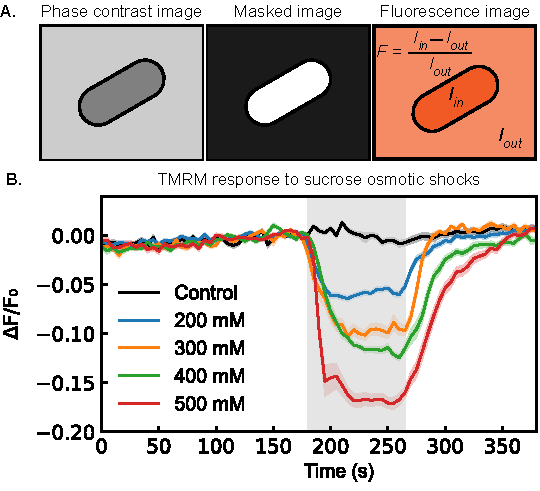
\includegraphics[width=0.6\linewidth]{figures/quantification_TMRM.pdf}
        \captionof{figure}{\footnotesize\revised{\textbf{Hyperosmotic shock induces transient membrane depolarization in \textit{E. coli}.}  \textbf{(A)} Schematic of the analysis pipeline for quantifying the TMRM signal. The cell image was segmented to generate a binary mask defining the intracellular region. The intracellular-to-extracellular fluorescence ratio $F = (I_{\mathrm{in}} - I_{\mathrm{out}})/I_{\mathrm{out}}$ was calculated from the mean fluorescence intensity inside the cell ($I_{\mathrm{in}}$), and the background intensity outside the cell ($I_{\mathrm{out}}$). \textbf{(B)} Population-averaged fluorescence ratios for 200--500~mM sucrose shocks and a 0~mM sucrose control ($n = 40$ per condition), normalized as $\Delta F/F_{0} = (F_{t} - F_{0})/F_{0}$, where $F_{t}$ is the fluorescence ratio at time $t$ and $F_{0}$ is the mean pre-shock value. Upon osmotic shock, fluorescence decreased in a dose-dependent manner and recovered to pre-shock values upon return to base media. Solid lines and shaded bands represent mean and SE.}}
        \label{fig:TMRM}
    \end{minipage}%
}
\end{center}

\end{mdframed}

\response{In the revised manuscript, we also include new data on cell size (measured as projected area) as a function of time during osmotic shock (Fig.~S5, reproduced below).} 

\setcounter{figure}{4}
\renewcommand{\thefigure}{S\arabic{figure}}

\begin{mdframed}
\begin{center}
\resizebox{0.95\linewidth}{!}{%
    \begin{minipage}{\linewidth}
        \centering
        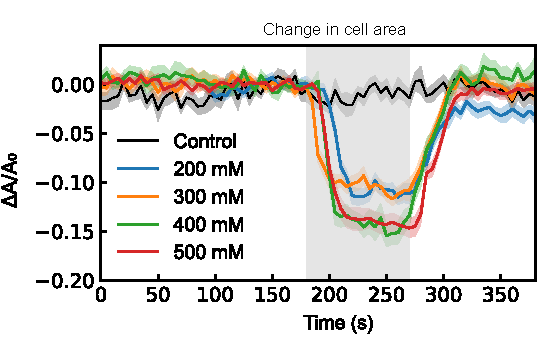
\includegraphics[width=0.6\linewidth]{figures/change-in-cell-area.pdf}
        \captionof{figure}{\footnotesize\revised{\textbf{Cell area decreases transiently following hyperosmotic shock.} Population-averaged fractional change in cell area during 200--500~mM sucrose shocks and a 0~mM sucrose control ($n$ = 40 per condition). MG1655 cells were grown to OD$_{600}$= 0.5, washed, and resuspended in a 1:10 dilution prior to imaging. Cell area was normalized as $\Delta A/A_{0} = (A_{t} - A_{0})/A_{0}$, where $A_{t}$ is the cell area at time $t$ and $A_{0}$ is the mean pre-shock value. Cell area decreased during the shock in a dose-dependent manner and recovered upon return to base media. Shaded regions indicate the duration of hyperosmotic exposure. Solid lines and shaded bands represent mean and SE, respectively.}}
    \label{sfig:cell-area}
    \end{minipage}%
}
\end{center}
\end{mdframed}

\item In Ref 42 by Rosko et al., it was found that weaker upshocks like 111 mOsmol/kg and 230 mOsmol/kg caused an increase in motor speed without a significant speed drop (see Fig. S2). This result seems inconsistent with the current study at 200 mM sucrose, which shows a rapid drop. Can the authors please: 1. explain the discrepancy; 2. use weaker hyperosmotic shocks and see if the results follow a similar trend as seen in Fig. 1D?

\response{We did not observe an increase in motor speed following osmotic shock at any concentration tested. Additional experiments using a weaker (100~mM sucrose) shock likewise showed a decrease in motor speed, consistent with our other data (Fig. S9, reproduced below). Several methodological differences may explain the discrepancy with Rosko et al. First, Rosko et al. used 0.5~$\mu$m beads whereas we used 1~$\mu$m beads; the smaller bead alters the mechanical load on the motor and could promote stator remodeling. Second, Rosko et al. manually pipetted media into a glass slide, whereas we used a syringe pump at a fixed flow rate of 15~mL/hr; manual handling may introduce shear stress and static media can alter the local microenvironment (e.g., oxygen availability), potentially affecting motor behavior. Third, Rosko et al. grew cultures to OD$_{600}$ = 0.8--1.0 compared to our OD$_{600}$ = 0.5--0.6; at higher cell densities PMF can decrease, which may further contribute to differences in motor behavior. Although osmoprotectants were present in the media of Rosko et al., adding osmoprotectants in our experiments did not increase motor speed after osmotic shock (Fig. S10, reproduced below), suggesting buffer composition alone does not account for the discrepancy.}
    
    
\response{We have added the following results on (p. 6):}

\begin{mdframed}
\footnotesize\revised{``These results differ from an earlier report in which motor speed increased above baseline following osmotic upshock at low shock magnitudes (43). We did not observe a speed increase at low osmolarities (Fig.~S2), nor did addition of osmoprotectants to the medium significantly affect our results~(Fig.~S3). Possible sources of this discrepancy are discussed later.'' (p. 6)}
\end{mdframed}

\setcounter{figure}{1}
\renewcommand{\thefigure}{S\arabic{figure}}
\begin{mdframed}
\begin{center}
\resizebox{0.95\linewidth}{!}{%
    \begin{minipage}{\linewidth}
        \centering
        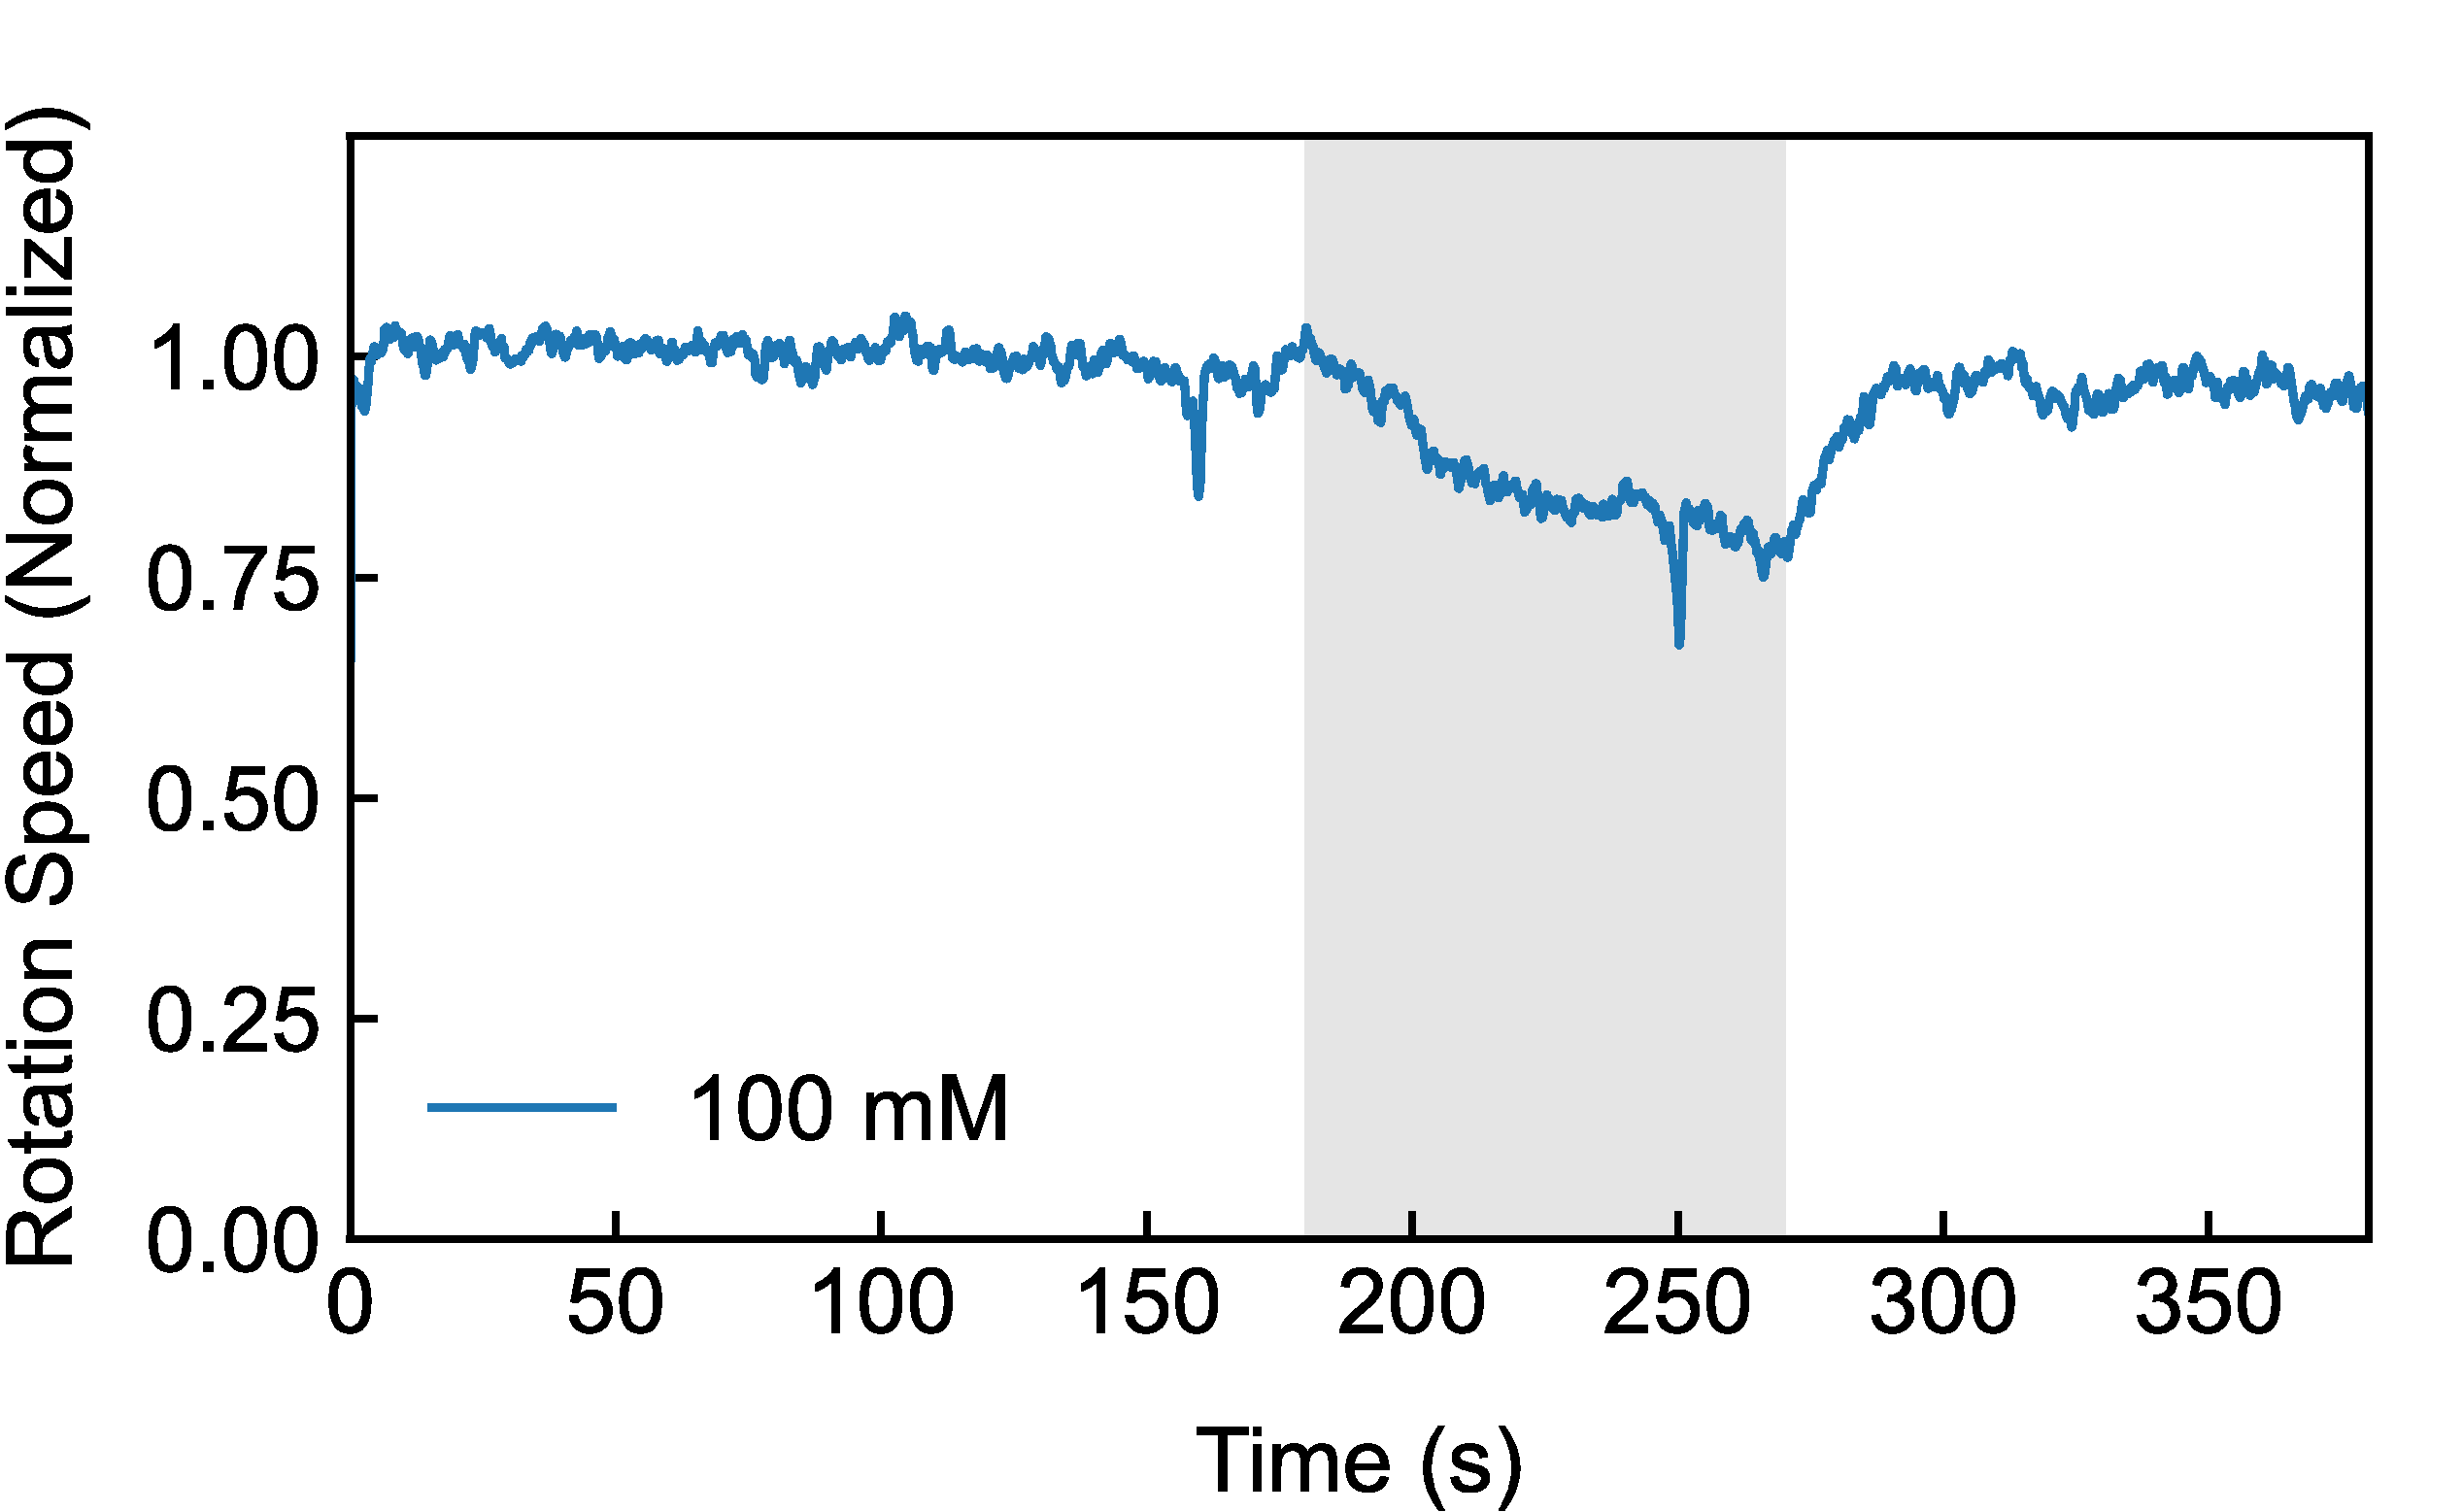
\includegraphics[width=0.7\linewidth]{figures/100mM.pdf}
        \captionof{figure}{\footnotesize\revised{\textbf{Motor speed decrease during a 100~mM hyperosmotic shock.} Population-averaged normalized rotation speed during exposure to 100~mM sucrose shock ($n$ = 9). Motor speed decreased upon addition of sucrose and remained reduced throughout the shock period, recovering upon return to base media. The shaded region indicates the duration of hyperosmotic exposure.}}
    \label{sfig:100mM-sucrose}
    \end{minipage}%
}
\end{center}
\end{mdframed}

\begin{mdframed}
\begin{center}
\resizebox{0.95\linewidth}{!}{%
    \begin{minipage}{\linewidth}
        \centering
        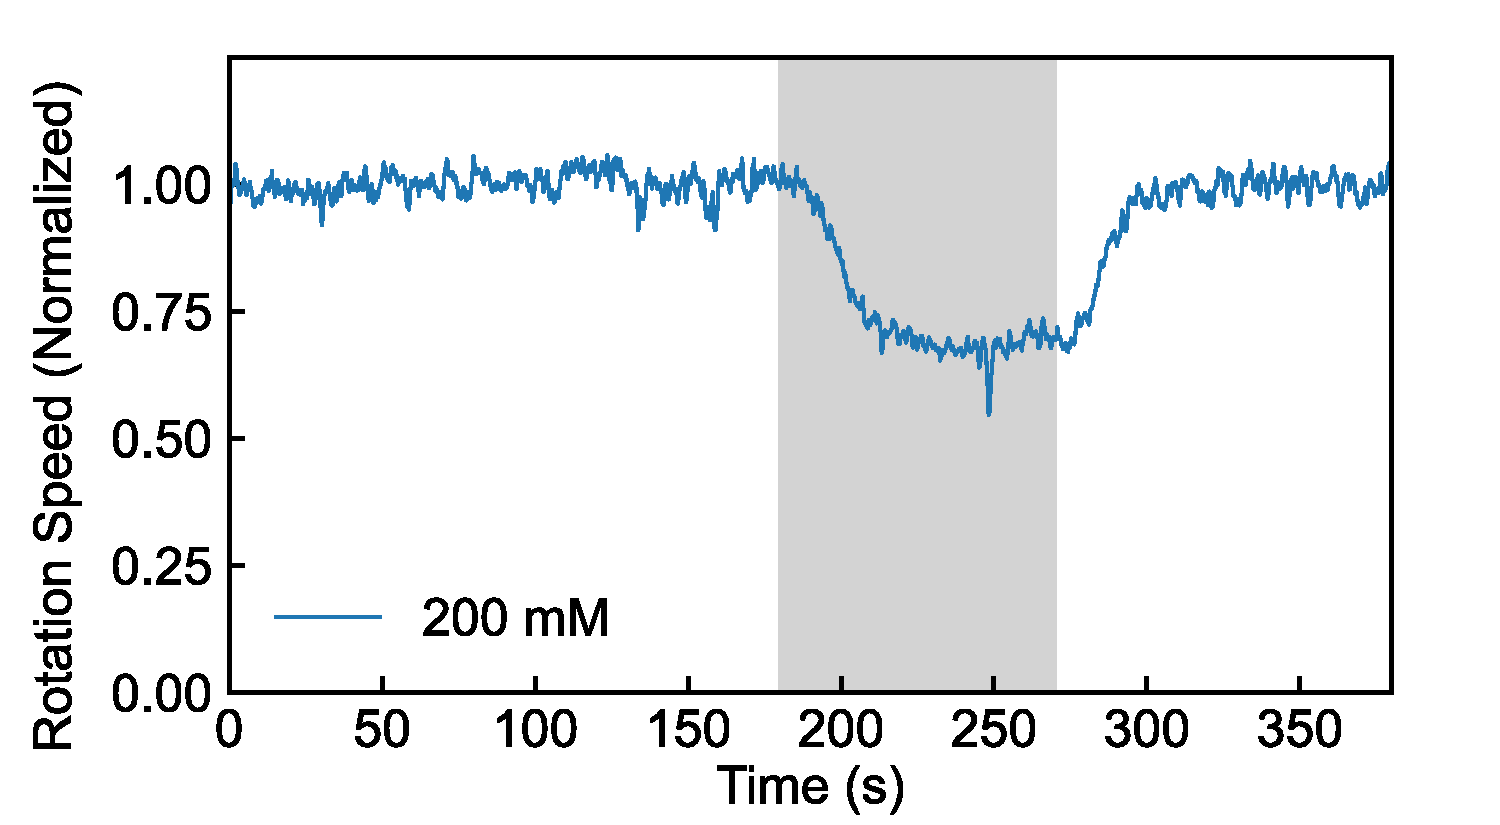
\includegraphics[width=0.7\linewidth]{figures/200-osmopro-short.pdf}
        \captionof{figure}{\footnotesize\revised{\textbf{Motor speed decreases during osmotic shock in the presence of osmoprotectants.} Population-averaged normalized rotation speed during exposure to 200~mM sucrose with osmoprotectants ($n$ = 9). Motor speed decreased upon addition of sucrose and did not recover during the shock period. The shaded region indicates the duration of hyperosmotic exposure.}}
    \label{sfig:200_short_osmopro}
    \end{minipage}%
}
\end{center}
\end{mdframed}

\response{We have also expanded the discussion (p. 9) to address these findings, adding the following text:}
    
\begin{mdframed}
\footnotesize\revised{``While our measurements consistently reveal a clear PMF decrease following hyperosmotic shock, our findings differ in an important respect from those of Rosko et al. (43), who reported an \textit{increase} in motor speed above baseline following osmotic upshock, with a transient speed drop observed at higher shock strengths. In contrast, we consistently observed a \textit{decrease} in motor speed, which we interpret as a reduction in PMF. Several methodological differences, including bead size, osmotic media delivery method, and flow cell geometry, may contribute to this discrepancy. Rosko et al. used 0.5~\textmu m beads, whereas we used 1~\textmu m beads, placing the motor at a different operating point on the torque-speed curve and potentially altering its response to PMF changes. The absence of any effect from the addition of osmoprotectants to our media argues against buffer composition as an explanation for the divergent results. Reconciling these differences represents an important open question for future work.'' (p. 9)}
\end{mdframed}

\item In the duration of the osmotic shock, the study does not find significant recovery of motor rotation speed or adaptation like that shown in Ref 42. Can the authors provide any comment or explanation for this difference? Is the result of Ref. 42 due to the presence of an osmoprotectant? If osmoprotectants were used here, would the authors reproduce the results in Ref. 42? These discussions/results will help clarify the mechanism.

\response{We repeated the sucrose shock experiments in the presence of osmoprotectants but did not find an increase in rotation speed following shock~(Figs.~S3, reproduced above).}

\response{As discussed above, the discrepancy between our results and those of Rosko et al. may arise from several experimental differences, including the initial motor load, the presence of quiescent media, manual exchange of media, and the higher optical densities of the cultures used in their experiments.}

\item Related to point 2, if the volume change can be measured, one can be more confident in associating PMF change with volume change, since Ref. 42 claimed that the length of the recovery phase roughly corresponds to the time cells take to recover the volume.
    
\response{As noted above, the revised manuscript includes new data on cell area as a function of time during osmotic shock (Fig. S6, reproduced above). Although the bead assays and cell-area measurements were performed on different cells, they used identical timing protocols, and both exhibit similar timescales, suggesting that changes in PMF and cell volume are coupled. This has been added to the main text (p. 6):}

\begin{mdframed}
\footnotesize\revised{These timescales are comparable to those of cell size changes following hyperosmotic shock (Fig. S6).}
\end{mdframed}

\item A discussion of the molecular mechanism behind the phenomena will be helpful.
    
\response{We thank the reviewer for their feedback and have expanded the discussion to address potential molecular mechanisms linking osmotic stress to PMF disruption:}

\begin{mdframed}
\footnotesize\revised{''While the precise molecular mechanism by which hyperosmotic shock disrupts membrane potential remains unclear, osmotic stress is known to broadly perturb cellular metabolism and respiration (66, 76, 77). Rapid inhibition of carbon uptake (76) and decreases in respiratory activity (66, 77) under osmotic stress suggest that proton-pumping processes may be transiently compromised. Hyperosmotic stress causes rapid water efflux through AqpZ (41, 42, 68), leading to cell shrinkage, changes in membrane tension (6, 39), and alterations in the cytoplasmic physicochemical state, including ionic strength, pH, and macromolecular crowding (70, 78–80). Changes in membrane tension could directly perturb the conformation and proton-pumping activity of ETC complexes embedded in the inner membrane; Complex I, for instance, undergoes conformational transitions linked to its catalytic state (81), and its activity may be sensitive to the lipid environment of the inner membrane (82, 83). Together these biophysical and metabolic perturbations could impair proton pumping and reduce membrane potential. The rapid timescale of motor slowdown observed here argues against transcriptional or translational responses, pointing instead toward an immediate biophysical or metabolic mechanism (68, 69). Mechanical perturbations have previously been shown to induce calcium influx and membrane depolarization in bacteria (8); however, this mechanism is unlikely to explain our observations, as our experimental media contained no calcium. Elucidating the mechanism linking osmotic stress to PMF disruption remains an important open question for future work.'' (p. 10).} 
\end{mdframed}
    
\end{itemize}

\section*{Reviewer 2} In this manuscript, Meneses et al. use the flagellar motor as a reporter to test the effect of hyperosmotic shock on PMF dynamics. They show that hyperosmotic shock causes a rapid, reversible collapse of PMF in E. coli. This is both an interesting result and a novel and innovative toolkit that could lead to further useful applications of the flagellar motor as a biosensor. The combination of biophysical/bioengineering techniques and relevance to a fascinating biomolecular system make this work of interest to the audience of Biophysical Journal, and in general I think it is a good fit. I do however have some concerns regarding mechanistic interpretation and clarity that I outline below.

\begin{itemize}
\item The core claim of the paper (that hyperosmotic shock leads to the collapse of PMF) is likely true. However, the PMF drop is inferred primarily from motor speed and TMRM fluorescence (which is largely qualitative). The dependence on motor speed for PMF quantification requires more care than is given by the authors, particularly given the possibility of stator remodeling and recent findings that the relationship between PMF and speed is not linear (e.g., Krasnopeeva et al., 2024). The authors quickly and briefly dismiss the possibility of stator remodeling, despite previous work suggesting PMF has a strong effect on stator occupancy. I would recommend either more rigorous analyses (e.g., via proper calibration and quantification of the TMRM signals) or that more cautious wording of their claims and addressing of the limitations in the Discussion are needed.

\response{We thank the reviewer for their constructive suggestions and have implemented both in the revised manuscript.}

\response{In response to concerns regarding TMRM quantification, we have substantially expanded our analysis. The revised manuscript now provides a quantitative treatment of the intracellular-to-extracellular TMRM fluorescence ratio (Fig.~2, reproduced below), with explicit normalization and background correction procedures. These measurements show a rapid, reproducible decrease in membrane potential following hyperosmotic shock, consistent with a reduction in PMF, and strengthen the link between the observed motor speed decrease and membrane depolarization.}

\setcounter{figure}{1}
\begin{mdframed}
\begin{center}
\resizebox{0.95\linewidth}{!}{%
    \begin{minipage}{\linewidth}
        \centering
        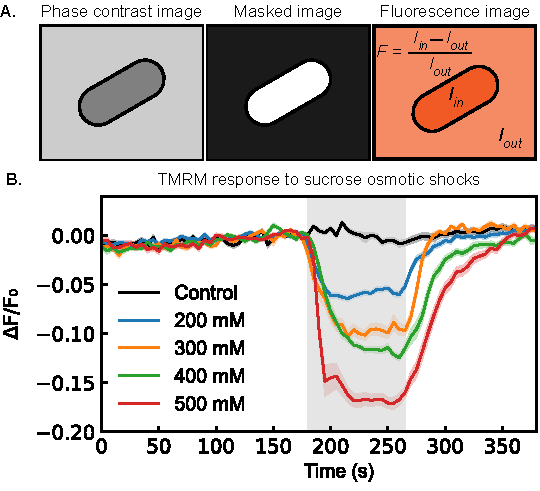
\includegraphics[width=0.6\linewidth]{figures/quantification_TMRM.pdf}
        \captionof{figure}{\footnotesize\revised{\textbf{Hyperosmotic shock induces transient membrane depolarization in \textit{E. coli}.}  \textbf{(A)} Schematic of the analysis pipeline for quantifying the TMRM signal. The cell image was segmented to generate a binary mask defining the intracellular region. The intracellular-to-extracellular fluorescence ratio $F = (I_{\mathrm{in}} - I_{\mathrm{out}})/I_{\mathrm{out}}$ was calculated from the mean fluorescence intensity inside the cell ($I_{\mathrm{in}}$), and the background intensity outside the cell ($I_{\mathrm{out}}$). \textbf{(B)} Population-averaged fluorescence ratios for 200--500~mM sucrose shocks and a 0~mM sucrose control ($n = 40$ per condition), normalized as $\Delta F/F_{0} = (F_{t} - F_{0})/F_{0}$, where $F_{t}$ is the fluorescence ratio at time $t$ and $F_{0}$ is the mean pre-shock value. Upon osmotic shock, fluorescence decreased in a dose-dependent manner and recovered to pre-shock values upon return to base media. Solid lines and shaded bands represent mean and SE.}}
        \label{fig:TMRM}
    \end{minipage}%
}
\end{center}
\end{mdframed}

\response{We have revised the corresponding section of the main text (p.~6) and expanded the discussion accordingly:}

\begin{mdframed}
\footnotesize\revised{``Our TMRM measurements provide independent support for the motor’s reliability as a reporter of PMF. At the external pH of $\sim$7.5 used in our experiments, $\Delta \text{pH}$ is negligible and the membrane potential therefore constitutes the dominant component of the PMF (48, 49). To minimize dye-induced perturbation of membrane potential, we used low TMRM concentrations that have been reported to reduce quenching, aggregation, and membrane disruption (29, 30). Under these conditions, the intracellular-to-extracellular fluorescence ratio decreased in a shock-dependent manner, mirroring the changes in motor speed. Thus, while motor measurements report on on flagellar rotation and TMRM assays report on dye distribution across the membrane, both independently indicate that that hyperosmotic shock depolarizes \textit{E. coli}.'' (p.~9)}
\end{mdframed}

\response{We have also revised the manuscript to expand the discussion of limitations and to be more precise in our wording. On p.~9, we clarify the dependence of motor speed on PMF:}

\begin{mdframed}
\footnotesize\revised{``Although the precise quantitative dependence of motor speed on PMF has been debated (33, 34, 64), the relationship is consistently monotonic,  making motor speed a reliable proxy for relative changes in PMF.'' (p. 9)} 
\end{mdframed}

\response{We have significantly expanded the discussion of stator remodeling and acknowledge the limitations of the present study on this point (p.~10):}

\begin{mdframed}
\footnotesize\revised{``PMF is known to regulate stator engagement with the motor (64, 71). However, both the decrease upon shock ($\sim 3\,\mathrm{s}$) and the recovery upon its removal ($\sim 3\,\mathrm{s}$) are far faster than reported timescales for stator disassembly and assembly, which range from $\sim10$ to $500\,\mathrm{s}$ under PMF-dependent or load-dependent remodeling conditions (71-75). For reference, sodium azide-induced stator disassembly occurs on a timescale of $\sim26\,\mathrm{s}$ (71), and stator assembly following load-dependent remodeling in the strain used here occurs on a timescale of $\sim50\,\mathrm{s}$ (74, 75), which are both at least an order of magnitude slower than the response we observe. Together, these comparisons suggest that stators likely remain bound throughout the osmotic shocks. However, since stator dynamics were not directly monitored in our experiments, remodeling cannot be formally ruled out. Whether the depolarization we observe leads to any stator rearrangement on longer timescales remains an open question.'' (p.~10)}
\end{mdframed}

\item The paper would be strengthened by more detailed discussion of the underlying mechanism. Hyperosmotic shock has a wide range of effects on bacterial physiology, several of which could affect PMF. The authors could expand the discussion to address such alternative explanations or weaken the language asserting a connection between a mechanical underlying cause for the PMF collapse during hyperosmotic shock.

\response{Thank you for this suggestion. In the revised manuscript, we have expanded the discussion of possible molecular mechanisms and tempered the language around a mechanical underlying cause:}

\begin{mdframed}
\footnotesize\revised{''While the precise molecular mechanism by which hyperosmotic shock disrupts membrane potential remains unclear, osmotic stress is known to broadly perturb cellular metabolism and respiration (66, 76, 77). Rapid inhibition of carbon uptake (76) and decreases in respiratory activity (66, 77) under osmotic stress suggest that proton-pumping processes may be transiently compromised. Hyperosmotic stress causes rapid water efflux through AqpZ (41, 42, 68), leading to cell shrinkage, changes in membrane tension (6, 39), and alterations in the cytoplasmic physicochemical state, including ionic strength, pH, and macromolecular crowding (70, 78–80). Changes in membrane tension could directly perturb the conformation and proton-pumping activity of ETC complexes embedded in the inner membrane; Complex I, for instance, undergoes conformational transitions linked to its catalytic state (81), and its activity may be sensitive to the lipid environment of the inner membrane (82, 83). Together these biophysical and metabolic perturbations could impair proton pumping and reduce membrane potential. The rapid timescale of motor slowdown observed here argues against transcriptional or translational responses, pointing instead toward an immediate biophysical or metabolic mechanism (68, 69). Mechanical perturbations have previously been shown to induce calcium influx and membrane depolarization in bacteria (8); however, this mechanism is unlikely to explain our observations, as our experimental media contained no calcium. Elucidating the mechanism linking osmotic stress to PMF disruption remains an important open question for future work.'' (p. 10).} 
\end{mdframed}

\item  TMRM imaging should be quantified in some manner. At the least, some population statistics should be provided.

\response{As described above, we have included new experiments and detailed quantification of the TMRM fluorescence (Fig. 2B and the related text).}

\end{itemize}

\noindent
Minor comments:

\begin{itemize}
\item Was there any measure or estimate of the media exchange time made? Some documentation of how this is calculated in the methods (not just in a citation) would be valuable.


\response{We have estimated the media exchange time experienced by the cell to be less than 1~s, and have added a brief note on this in the Discussion (p.~10), with the detailed calculation provided in the Supplemental Material.}

\begin{mdframed}
\revised{''The characteristic timescale of motor speed decrease is a few seconds (Fig. S4), and because the estimated media exchange time is much shorter ($\sim400~\textrm{ms}$; see Supporting Information), this reflects the intrinsic cellular response rather than the kinetics of the delivery of osmotic shock.'' (p. 10)}
\end{mdframed}

\item Strain descriptions should be more detailed for all strains used.

\response{We have added additional strain details to the Materials and Methods (p.~2).}

\item Normalization procedures should be stated explicitly in the relevant figure captions. Unnormalized plots should ideally be available in the supplementary information.

\response{Normalization procedures are now stated explicitly in the relevant figure captions, and unnormalized plots are included in the Supplemental Material (Fig.~S1).}

\item TMRM images should have intensity scale bars for proper comparison between images.

\response{In the revised manuscript, we replace the qualitative TMRM fluorescence images with quantitative plots of the intracellular-to-extracellular fluorescence ratio as a function of time following osmotic shock, enabling a more rigorous comparison across conditions (Fig.~2B).}

\end{itemize}

\section*{Reviewer 3} In their manuscript entitled "Omotic stress triggers fast and reversible PMF collapse in Escherichia coli," the authors use rotation of the flagellar motor as a read-out for membrane bioenergetics during exposure to and recovery from osmotic stress. They observe that exposure to hyperosmotic shocks results in decreased flagellar rotation (i.e., reduced PMF), with the magnitude of change proportional to the intensity of the shock. The experiments were performed under conditions where $\Delta$pH is expected to have negligible effects on PMF, so the observed differences are almost certainly due to alterations in membrane potential. The presumed changes in membrane potential are likely independent of either K+ or Ca2+ flux, although the exact mechanism that underlies them remains to be identified.

Altogether, this study is experimentally sound and reports relevant data regarding how bacteria respond to a critical environmental stress condition. The use of flagellar rotation is a clever way to assay real-time membrane energetics in a minimally invasive manner.

\begin{itemize}
\item Additional information should be reported in conjunction with Fig 2 to support and strengthen claims of decreased membrane potential.
\begin{itemize}

\item Quantification of the TMRM fluorescence before and after osmotic shock is needed to accurately report that membrane potential is in fact decreased. The supplemental figure associated with Fig 2 also has cells that appear to have unchanged fluorescence intensity throughout the experiment. The text acknowledges heterogeneity in fluorescence intensity, but this is an easily quantifiable metric.

    
\response{The revised manuscript includes new TMRM fluorescence measurements during osmotic shock (Fig.~2B, reproduced below), using improved labeling procedures that mitigate heterogeneous staining. We now provide quantitative analysis of the intracellular-to-extracellular fluorescence ratio over time rather than qualitative images, and observe a rapid decrease in this ratio upon shock, indicating a reduction in membrane potential consistent with PMF disruption.}

\response{These results have been added to the manuscript (p.~6), with expanded discussion on p.~9:}

\begin{mdframed}
\footnotesize\revised{``Our TMRM measurements provide independent support for the motor’s reliability as a reporter of PMF. At the external pH of $\sim$7.5 used in our experiments, $\Delta \text{pH}$ is negligible and the membrane potential therefore constitutes the dominant component of the PMF (48, 49). To minimize dye-induced perturbation of membrane potential, we used low TMRM concentrations that have been reported to reduce quenching, aggregation, and membrane disruption (29, 30). Under these conditions, the intracellular-to-extracellular fluorescence ratio decreased in a shock-dependent manner, mirroring the changes in motor speed. Thus, while motor measurements report on on flagellar rotation and TMRM assays report on dye distributi   on across the membrane, both independently indicate that that hyperosmotic shock depolarizes \textit{E. coli}.'' (p. 9)}
\end{mdframed}

\setcounter{figure}{1}
\begin{mdframed}
\begin{center}
\resizebox{0.95\linewidth}{!}{%
    \begin{minipage}{\linewidth}
        \centering
        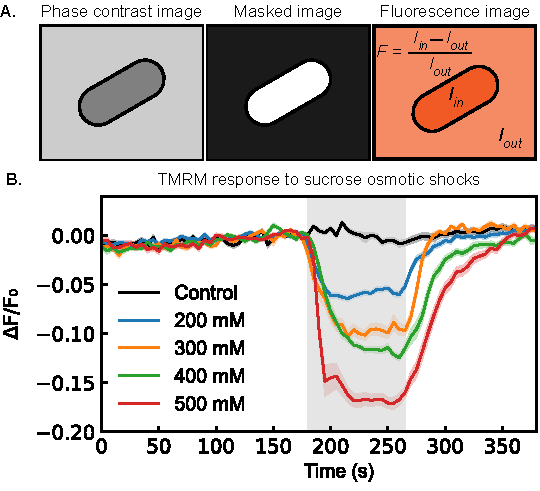
\includegraphics[width=0.6\linewidth]{figures/quantification_TMRM.pdf}
        \captionof{figure}{\footnotesize\revised{\textbf{Hyperosmotic shock induces transient membrane depolarization in \textit{E. coli}.}  \textbf{(A)} Schematic of the analysis pipeline for quantifying the TMRM signal. The cell image was segmented to generate a binary mask defining the intracellular region. The intracellular-to-extracellular fluorescence ratio $F = (I_{\mathrm{in}} - I_{\mathrm{out}})/I_{\mathrm{out}}$ was calculated from the mean fluorescence intensity inside the cell ($I_{\mathrm{in}}$), and the background intensity outside the cell ($I_{\mathrm{out}}$). \textbf{(B)} Population-averaged fluorescence ratios for 200--500~mM sucrose shocks and a 0~mM sucrose control ($n = 40$ per condition), normalized as $\Delta F/F_{0} = (F_{t} - F_{0})/F_{0}$, where $F_{t}$ is the fluorescence ratio at time $t$ and $F_{0}$ is the mean pre-shock value. Upon osmotic shock, fluorescence decreased in a dose-dependent manner and recovered to pre-shock values upon return to base media. Solid lines and shaded bands represent mean and SE.}}
        \label{fig:TMRM}
    \end{minipage}%
}
\end{center}
\end{mdframed}

\item It would be more informative to report the exact time points of when images were captured instead of "Before/During/After" labels. For example, are all "During" images captured at the same point in exposure to hyperosmotic stress? The cell in the fourth and fifth panels of Fig 2 appears to undergo some morphological alterations during the stress exposure that not all cells experienced. It is unclear if the exposure time of the cells in these panels are the same as others?

\response{Fig.~2, reproduced above, now shows full time series of the TMRM fluorescence ratio, with measurements collected every 5 seconds. The fourth and fifth panel of the previous Fig.~2 showed significant cell deformation due to higher levels of osmotic stress.}
    
\response{The revised manuscript also includes new measurements of cell area as a function of time during osmotic shock (Fig.~S5, reproduced below), which have been added to the main text (p.~6):}

\begin{mdframed}
    \footnotesize\revised{These timescales are comparable to those of cell size changes following hyperosmotic shock (Fig.~S5).}
\end{mdframed}

\setcounter{figure}{4}
\renewcommand{\thefigure}{S\arabic{figure}}
\begin{mdframed}
\begin{center}
\resizebox{0.95\linewidth}{!}{%
    \begin{minipage}{\linewidth}
        \centering
        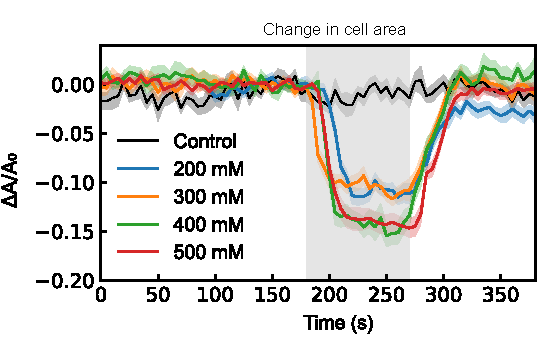
\includegraphics[width=0.7\linewidth]{figures/change-in-cell-area.pdf}
        \captionof{figure}{\footnotesize\revised{\textbf{Cell area decreases transiently following hyperosmotic shock.} Population-averaged fractional change in cell area during 200--500~mM sucrose shocks and a 0~mM sucrose control ($n$ = 40 per condition). MG1655 cells were grown to OD$_{600}$= 0.5, washed, and resuspended in a 1:10 dilution prior to imaging. Cell area was normalized as $\Delta A/A_{0} = (A_{t} - A_{0})/A_{0}$, where $A_{t}$ is the cell area at time $t$ and $A_{0}$ is the mean pre-shock value. Cell area decreased during the shock in a dose-dependent manner and recovered upon return to base media. Shaded regions indicate the duration of hyperosmotic exposure. Solid lines and shaded bands represent mean and SE, respectively.}}
    \label{sfig:cell-area}
    \end{minipage}%
}
\end{center}

\end{mdframed}
\end{itemize}

\item The authors determine that the presumed membrane potential changes are likely independent of K+ or Ca2+ and suggest that the depolarization could be a result of ETC disruption. Would an ETC mutant or performing the experiment in the presence of an ETC-impairing compound (i.e., potassium cyanide) help confirm this hypothesis? What about the potential involvement of ion or mechanosensitive channels?

\response{We thank the reviewer for this thoughtful suggestion. ETC mutants could indeed help test whether osmotic stress impairs ETC function and thereby reduces PMF. However, generating and validating such mutants would require substantial cloning and optimization effort, particularly given the essential role of the ETC in cellular physiology, and chemical inhibition of the ETC may not faithfully recapitulate the physical perturbations induced by osmotic shock. We therefore did not pursue these experiments in the present study, but investigating the role of the ETC in the osmotic stress response remains an important direction for future work.}

\item The authors discuss how the potential conflict of their data with previous studies where no changes in PMF were reported could be due to differences in time scales. Prior data reported on changes after minutes of exposure, whereas data reported here is on the second level. Could the rotational measurements during exposure to hyperosmotic stress be extended to 2-3 min to confirm?

\response{We extended the duration of osmotic shocks to test whether adaptation occurs over longer timescales. When cells were maintained in hyperosmotic medium for an extended period, motor speed recovered to levels consistent with the viscosity predictions (Fig.~6, reproduced below), indicating that PMF returns to approximately its pre-shock value following adaptation. The residual reduction in motor speed is largely accounted for by the increased viscous load of the sucrose solution. Studies using longer incubation protocols may therefore have missed the transient PMF drop and recovery that occurs within the first few minutes after shock.}

\response{These results have been added to the main text {(p.~8)} and further discussed on p.~{10}.}

 \setcounter{figure}{5}
\begin{mdframed}

\begin{center}
\resizebox{0.95\linewidth}{!}{%
    \begin{minipage}{\linewidth}
        \centering
        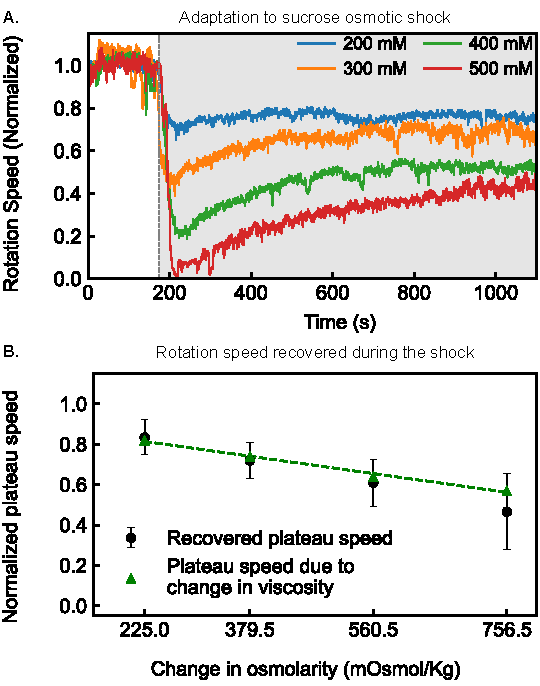
\includegraphics[width=0.6\linewidth]{figures/osmoadaption-biophysics.pdf}
        \captionof{figure}{\footnotesize\revised{\textbf{Adaptation of flagellar motor speed following hyperosmotic shock.} 
    \textbf{(A)} Time courses of normalized flagellar motor rotation speed after application of sucrose osmotic shocks of different magnitudes (200--500 mM). The dashed vertical line indicates the time at which the hyperosmotic medium was introduced. Motor speed drops rapidly following the shock and then partially recovers over several minutes to a new steady plateau whose level depends on the shock strength. Traces represent the mean of $n = 8, 8, 8,$ and $4$ motors for 200~mM, 300~mM, 400~mM, and 500~mM sucrose upshifts, respectively, normalized to the pre-shock speed.
    \textbf{(B)} Plateau motor speed measured several minutes after the shock as a function of the change in osmolarity. Black circles and black error bars represent the mean and SD, respectively. Green triangles indicate the plateau speed expected from the increase in medium viscosity due to sucrose alone.}}
        \label{fig:osmoadaption}
    \end{minipage}%
}
\end{center}
\end{mdframed}

\begin{mdframed}
\footnotesize\revised{On longer timescales, our sustained shock experiments reveals that PMF recovers over several minutes --- dynamics that were likely missed in earlier studies reporting no significant changes in PMF several minutes after shock (66, 67). This recovery timescale is consistent with that of cellular volume recovery following osmotic shock (43, 65), suggesting that the two processes are coupled. Since protein synthesis occurs on longer timescales than those we observe~(68, 69) PMF recovery is most likely mediated by pre-existing adaptation mechanisms~(39, 41, 70) rather than new protein production.'' (p. 10)}
\end{mdframed}
\end{itemize}

\end{document}